\documentclass[12pt, a4paper]{article}

% --- Pacotes ---
\usepackage[utf8]{inputenc}
\usepackage[T1]{fontenc}
\usepackage[brazil]{babel}
\usepackage{amsmath, amssymb}
\usepackage{graphicx}
\usepackage{booktabs}
\usepackage{array}
\usepackage{caption}
\usepackage{subcaption}
\usepackage{hyperref}
\usepackage{geometry}
\usepackage{float}
\usepackage{algorithm}
\usepackage{algpseudocode}
\graphicspath{{../../graficos/}{graficos/}}
\geometry{margin=2.5cm}

\title{Resolução do Problema do Caixeiro Viajante com Heurísticas Construtivas}
\author{Bernardo Vale dos Santos Bento}
\date{16/09/2026}

\begin{document}

\maketitle

% -------------------------------------------------------
\section{Visão Geral do Projeto}
% -------------------------------------------------------

O Problema do Caixeiro Viajante (\textit{Traveling Salesman Problem} --- TSP) consiste em
encontrar o circuito hamiltoniano de menor custo que visita todos os vértices de um grafo
exatamente uma vez e retorna ao vértice de partida. Por ser um problema NP-Difícil
(\textit{NP-Hard}), métodos exatos tornam-se intratáveis à medida que o número de vértices
cresce, demandando o uso de \textbf{heurísticas construtivas} capazes de entregar boas
soluções em tempo polinomial.

Este projeto implementou um \textit{framework} em Python que:
\begin{enumerate}
    \item \textbf{Lê instâncias padrão TSPLIB}: suporta as formulações de pesos de arestas
          \texttt{EUC\_2D} (distância euclidiana bidimensional) e \texttt{ATT} (distância
          pseudo-euclidiana com correção inteira).
    \item \textbf{Avalia 6 Heurísticas Construtivas}:
          \begin{itemize}
              \item \textbf{3 Heurísticas Autorais} (foram modeladas pelo autor sem conhecimento externo, o que não impede delas já existirem): \textit{Centroid-Based Insertion} (H1),
                    \textit{Eccentricity Insertion} (H2) e \textit{Hybrid-Score Insertion} (H3).
              \item \textbf{3 Heurísticas Clássicas da Literatura}: \textit{Nearest Neighbor}
                    (H4) \cite{rosenkrantz1977}, \textit{Farthest Insertion} (H5)
                    \cite{rosenkrantz1977} e \textit{Greedy Edge} (H6) \cite{bentley1992}.
          \end{itemize}
    \item \textbf{Mede e Compara Desempenho}: coleta tempo de execução computacional em
          milissegundos ($ms$) e custo final do circuito percorrido em 21 instâncias
          \textit{benchmark}.
    \item \textbf{Visualização Estatística}: gera gráficos estilo \textit{boxplot} com caso
          médio, \textit{heatmaps} comparativos (custo relativo e tempo) e análise de
          dominância via Fronteira de Pareto.
\end{enumerate}

% -------------------------------------------------------
\section{Modelagem e Fórmulas de Distância}
% -------------------------------------------------------

As coordenadas dos vértices $(x_i, y_i)$ são lidas e mantidas com precisão contínua em
ponto flutuante (\texttt{float}). O cálculo das distâncias entre dois vértices $i$ e $j$
segue rigorosamente a especificação oficial da TSPLIB:

\subsection{Distância Pseudo-Euclidiana (\texttt{ATT})}

Utilizada na instância \texttt{att48.tsp}:

\begin{equation}
    \Delta x = x_i - x_j, \qquad \Delta y = y_i - y_j
\end{equation}
\begin{equation}
    r_{ij} = \sqrt{\frac{\Delta x^2 + \Delta y^2}{10{,}0}}
\end{equation}
\begin{equation}
    t_{ij} = \mathrm{nint}(r_{ij})
\end{equation}
\begin{equation}
    d_{ij} =
    \begin{cases}
        t_{ij} + 1, & \text{se } t_{ij} < r_{ij} \\
        t_{ij},     & \text{caso contrário}
    \end{cases}
\end{equation}

\noindent onde $\mathrm{nint}(z) = \lfloor z + 0{,}5 \rfloor$.

\subsection{Distância Euclidiana 2D (\texttt{EUC\_2D})}

Utilizada nas demais instâncias:

\begin{equation}
    d_{ij} = \mathrm{nint}\!\left(\sqrt{(x_i - x_j)^2 + (y_i - y_j)^2}\right)
\end{equation}

% -------------------------------------------------------
\section{Definição das Métricas de Avaliação}
% -------------------------------------------------------

Para comparar as heurísticas de forma justa entre instâncias de tamanhos e escalas
distintos, definem-se as seguintes métricas:

\paragraph{Custo Médio Absoluto.}
Média aritmética dos comprimentos dos circuitos gerados pela heurística $h$ ao longo das
21 instâncias avaliadas:

\begin{equation}
    \overline{C}(h) = \frac{1}{21} \sum_{i=1}^{21} C(h, \mathcal{I}_i)
\end{equation}

\noindent onde $C(h, \mathcal{I}_i)$ é o custo do circuito produzido pela heurística $h$
na instância $\mathcal{I}_i$.

\paragraph{Custo Relativo e Custo Médio Relativo.}
Para cada instância $\mathcal{I}_i$, define-se o \textbf{Custo Relativo} de uma
heurística $h$ como a razão entre o custo obtido por $h$ e o melhor custo encontrado
por qualquer heurística naquela instância:

\begin{equation}
    \mathrm{CR}(h, \mathcal{I}_i)
    = \frac{C(h, \mathcal{I}_i)}{\displaystyle\min_{h'} C(h', \mathcal{I}_i)}
\end{equation}

\noindent Por construção, $\mathrm{CR}(h, \mathcal{I}_i) \geq 1{,}000$, sendo igual a
$1{,}000$ quando $h$ produz a melhor solução naquela instância. O \textbf{Custo Médio
Relativo} agrega esse indicador sobre todas as instâncias:

\begin{equation}
    \overline{\mathrm{CR}}(h)
    = \frac{1}{21} \sum_{i=1}^{21} \mathrm{CR}(h, \mathcal{I}_i)
\end{equation}

% -------------------------------------------------------
\section{Heurísticas Autorais}
% -------------------------------------------------------

Todas as três heurísticas propostas baseiam-se na técnica de
\textbf{Inserção Mais Barata} (\textit{Cheapest Insertion}). Dado um circuito parcial,
o custo marginal de inserir o vértice $v$ na aresta $(i,j)$ é:

\begin{equation}
    \Delta(i, v, j) = d(i,v) + d(v,j) - d(i,j)
    \label{eq:cheapest}
\end{equation}

A inserção de $v$ é sempre realizada na aresta $(i,j)$ que minimiza
$\Delta(i,v,j)$. A inovação das três heurísticas reside no critério de
\textbf{ordenação e priorização} dos vértices a serem inseridos.

% --- H1 ---
\subsection{H1 --- \textit{Centroid-Based Insertion}}

\paragraph{Motivação geométrica.}
Em problemas euclidianos, vértices localizados na periferia da nuvem de pontos possuem
poucas alternativas de arestas sem cruzar o interior do grafo. Se deixados para o final,
inserir esses vértices força o circuito a esticar arestas já consolidadas através de
grandes distâncias, gerando cruzamentos graves. Ao construir primeiro o ``esqueleto''
externo formado pelos nós periféricos, os vértices internos são absorvidos com desvios
locais mínimos.

\paragraph{Algoritmo.}
\begin{enumerate}
    \item Calcula o centróide médio das coordenadas:
          \begin{equation}
              \mathbf{C} = \left(\frac{1}{n}\sum_{i=1}^n x_i,\;
                                  \frac{1}{n}\sum_{i=1}^n y_i\right)
          \end{equation}
    \item Atribui a cada vértice $v$ a prioridade:
          \begin{equation}
              \mathrm{prioridade}(v) = d(v, \mathbf{C})
          \end{equation}
    \item Ordena todos os vértices em ordem \textbf{decrescente} de prioridade.
    \item Inicia o circuito com os 2 vértices mais distantes do centróide e insere os
          demais via \textit{cheapest insertion} (Equação~\ref{eq:cheapest}).
\end{enumerate}

% --- H2 ---
\subsection{H2 --- \textit{Eccentricity Insertion}}

\paragraph{Motivação topológica.}
A heurística H1 depende da existência e representatividade de coordenadas cartesianas
$(x, y)$. Para instâncias cujas distâncias provêm de matrizes arbitrárias ou espaços
não-euclidianos, o conceito de centróide geométrico perde o sentido. A excentricidade
captura a noção de ``periferia'' puramente a partir da matriz de distâncias: vértices com
alta soma de distâncias estão na borda do grafo e devem ser fixados no circuito logo no
início.

\paragraph{Algoritmo.}
\begin{enumerate}
    \item Calcula a excentricidade de cada vértice $v$:
          \begin{equation}
              \mathrm{exc}(v) = \sum_{\substack{u \in V \\ u \neq v}} d(v, u)
          \end{equation}
    \item Define $\mathrm{prioridade}(v) = \mathrm{exc}(v)$.
    \item Ordena os vértices em ordem \textbf{decrescente} de excentricidade.
    \item Inicia com os 2 vértices mais excêntricos e insere os restantes via
          \textit{cheapest insertion}.
\end{enumerate}

% --- H3 ---
\subsection{H3 --- \textit{Hybrid-Score Insertion} ($\alpha = \beta = 0{,}5$)}

\paragraph{Motivação.}
Une a intuição espacial explícita de H1 com a informação global da malha de distâncias
de H2. A combinação direta das duas métricas, no entanto, é inadmissível sem
normalização: a distância ao centróide é da ordem $O(L)$, enquanto a excentricidade é
da ordem $O(n \cdot L)$, de modo que a soma sem escala faria H2 dominar a decisão
integralmente.

\paragraph{Algoritmo.}
\begin{enumerate}
    \item Normaliza ambas as grandezas para o intervalo $[0, 1]$:
          \begin{equation}
              \mathrm{norm}(X) = \frac{X - X_{\min}}{X_{\max} - X_{\min}}
          \end{equation}
    \item Calcula o \textit{score} ponderado com $\alpha = \beta = 0{,}5$:
          \begin{equation}
              \mathrm{score}(v) =
              0{,}5 \cdot \mathrm{norm}\!\left(d(v, \mathbf{C})\right)
              + 0{,}5 \cdot \mathrm{norm}\!\left(\mathrm{exc}(v)\right)
          \end{equation}
    \item Ordena em ordem \textbf{decrescente} do \textit{score} e insere via
          \textit{cheapest insertion}.
\end{enumerate}

% -------------------------------------------------------
\section{Heurísticas da Literatura}
% -------------------------------------------------------

\subsection{H4 --- \textit{Nearest Neighbor} \cite{rosenkrantz1977}}

Começa em um vértice arbitrário e constrói o circuito de forma gulosa, sempre avançando
para o vértice não visitado mais próximo do atual. Ao final, fecha o circuito retornando
ao vértice de origem. Apesar de sua simplicidade e complexidade $O(n^2)$, a heurística
tende a produzir rotas com custo entre 20\% e 25\% acima do ótimo, pois as arestas de
fechamento forçadas ao final costumam ser longas.

\subsection{H5 --- \textit{Farthest Insertion} \cite{rosenkrantz1977}}

Inicializa o circuito com o par de vértices de maior distância mútua. A cada iteração,
identifica o vértice $k$ fora do circuito cuja distância mínima até qualquer vértice já
presente na rota é máxima --- isto é, o vértice mais ``isolado'' em relação ao circuito
atual --- e o insere na posição de menor custo marginal via \textit{cheapest insertion}.
Considerada na literatura uma das melhores heurísticas construtivas puras para o TSP,
com desvio médio em torno de 15\% a 20\% do ótimo \cite{rosenkrantz1977}.

\subsection{H6 --- \textit{Greedy Edge} \cite{bentley1992}}

Ordena todas as $\binom{n}{2}$ arestas do grafo completo por custo crescente. Em seguida,
percorre essa lista e adiciona cada aresta ao conjunto solução se, e somente se, forem
satisfeitas três condições: (i) nenhum dos dois vértices da aresta possui grau 2 no
conjunto já construído; (ii) a adição não cria um subtour prematuro (verificado via
estrutura \textit{Union-Find}); e (iii) não é a última aresta antes de fechar o ciclo
completo de $n$ vértices. A complexidade é dominada pela ordenação inicial,
resultando em $O(n^2 \log n)$.

% -------------------------------------------------------
\section{Resultados Numéricos}
% -------------------------------------------------------

A Tabela~\ref{tab:resultados} apresenta o resumo das métricas computadas em 21 instâncias
\textit{benchmark} da TSPLIB, com número de vértices variando de 48 (\texttt{att48}) a
200 (\texttt{kroA200}, \texttt{kroB200}).

\begin{table}[H]
    \centering
    \caption{Resumo de desempenho das 6 heurísticas em 21 instâncias.}
    \label{tab:resultados}
    \resizebox{\textwidth}{!}{%
    \begin{tabular}{lcccc}
        \toprule
        \textbf{Heurística}
            & \textbf{Custo Médio Absoluto}
            & \textbf{Custo Médio Relativo}
            & \textbf{Tempo Médio (ms)}
            & \textbf{Observação} \\
        \midrule
        H5 --- \textit{Farthest Insertion}
            & 35.429 & 1,002 & 5,99 & Melhor qualidade média \\
        H1 --- \textit{Centroid-Based}
            & 36.292 & 1,038 & 3,33 & Melhor custo-benefício \\
        H2 --- \textit{Eccentricity}
            & 36.335 & 1,038 & 5,17 & Agnóstica a coordenadas \\
        H3 --- \textit{Hybrid-Score}
            & 36.395 & 1,039 & 5,25 & Alta robustez combinada \\
        H6 --- \textit{Greedy Edge}
            & 39.437 & 1,097 & 4,87 & Qualidade intermediária \\
        H4 --- \textit{Nearest Neighbor}
            & 41.117 & 1,161 & 1,25 & Mais rápida; pior qualidade \\
        \bottomrule
    \end{tabular}}
\end{table}

Os resultados evidenciam que H5 produz o menor custo médio absoluto, enquanto H1
apresenta o melhor equilíbrio entre qualidade de solução e tempo de execução --- sendo
quase duas vezes mais rápida que H5 com apenas $\approx 3{,}6\%$ de diferença no custo
médio relativo. As heurísticas autorais H1, H2 e H3 superam consistentemente H4 e H6,
operando na faixa de 3,8\% a 3,9\% acima do melhor resultado por instância.

% -------------------------------------------------------
\section{Análise dos Gráficos}
% -------------------------------------------------------

\subsection{\textit{Heatmap} de Qualidade da Solução}

\begin{figure}[H]
    \centering
    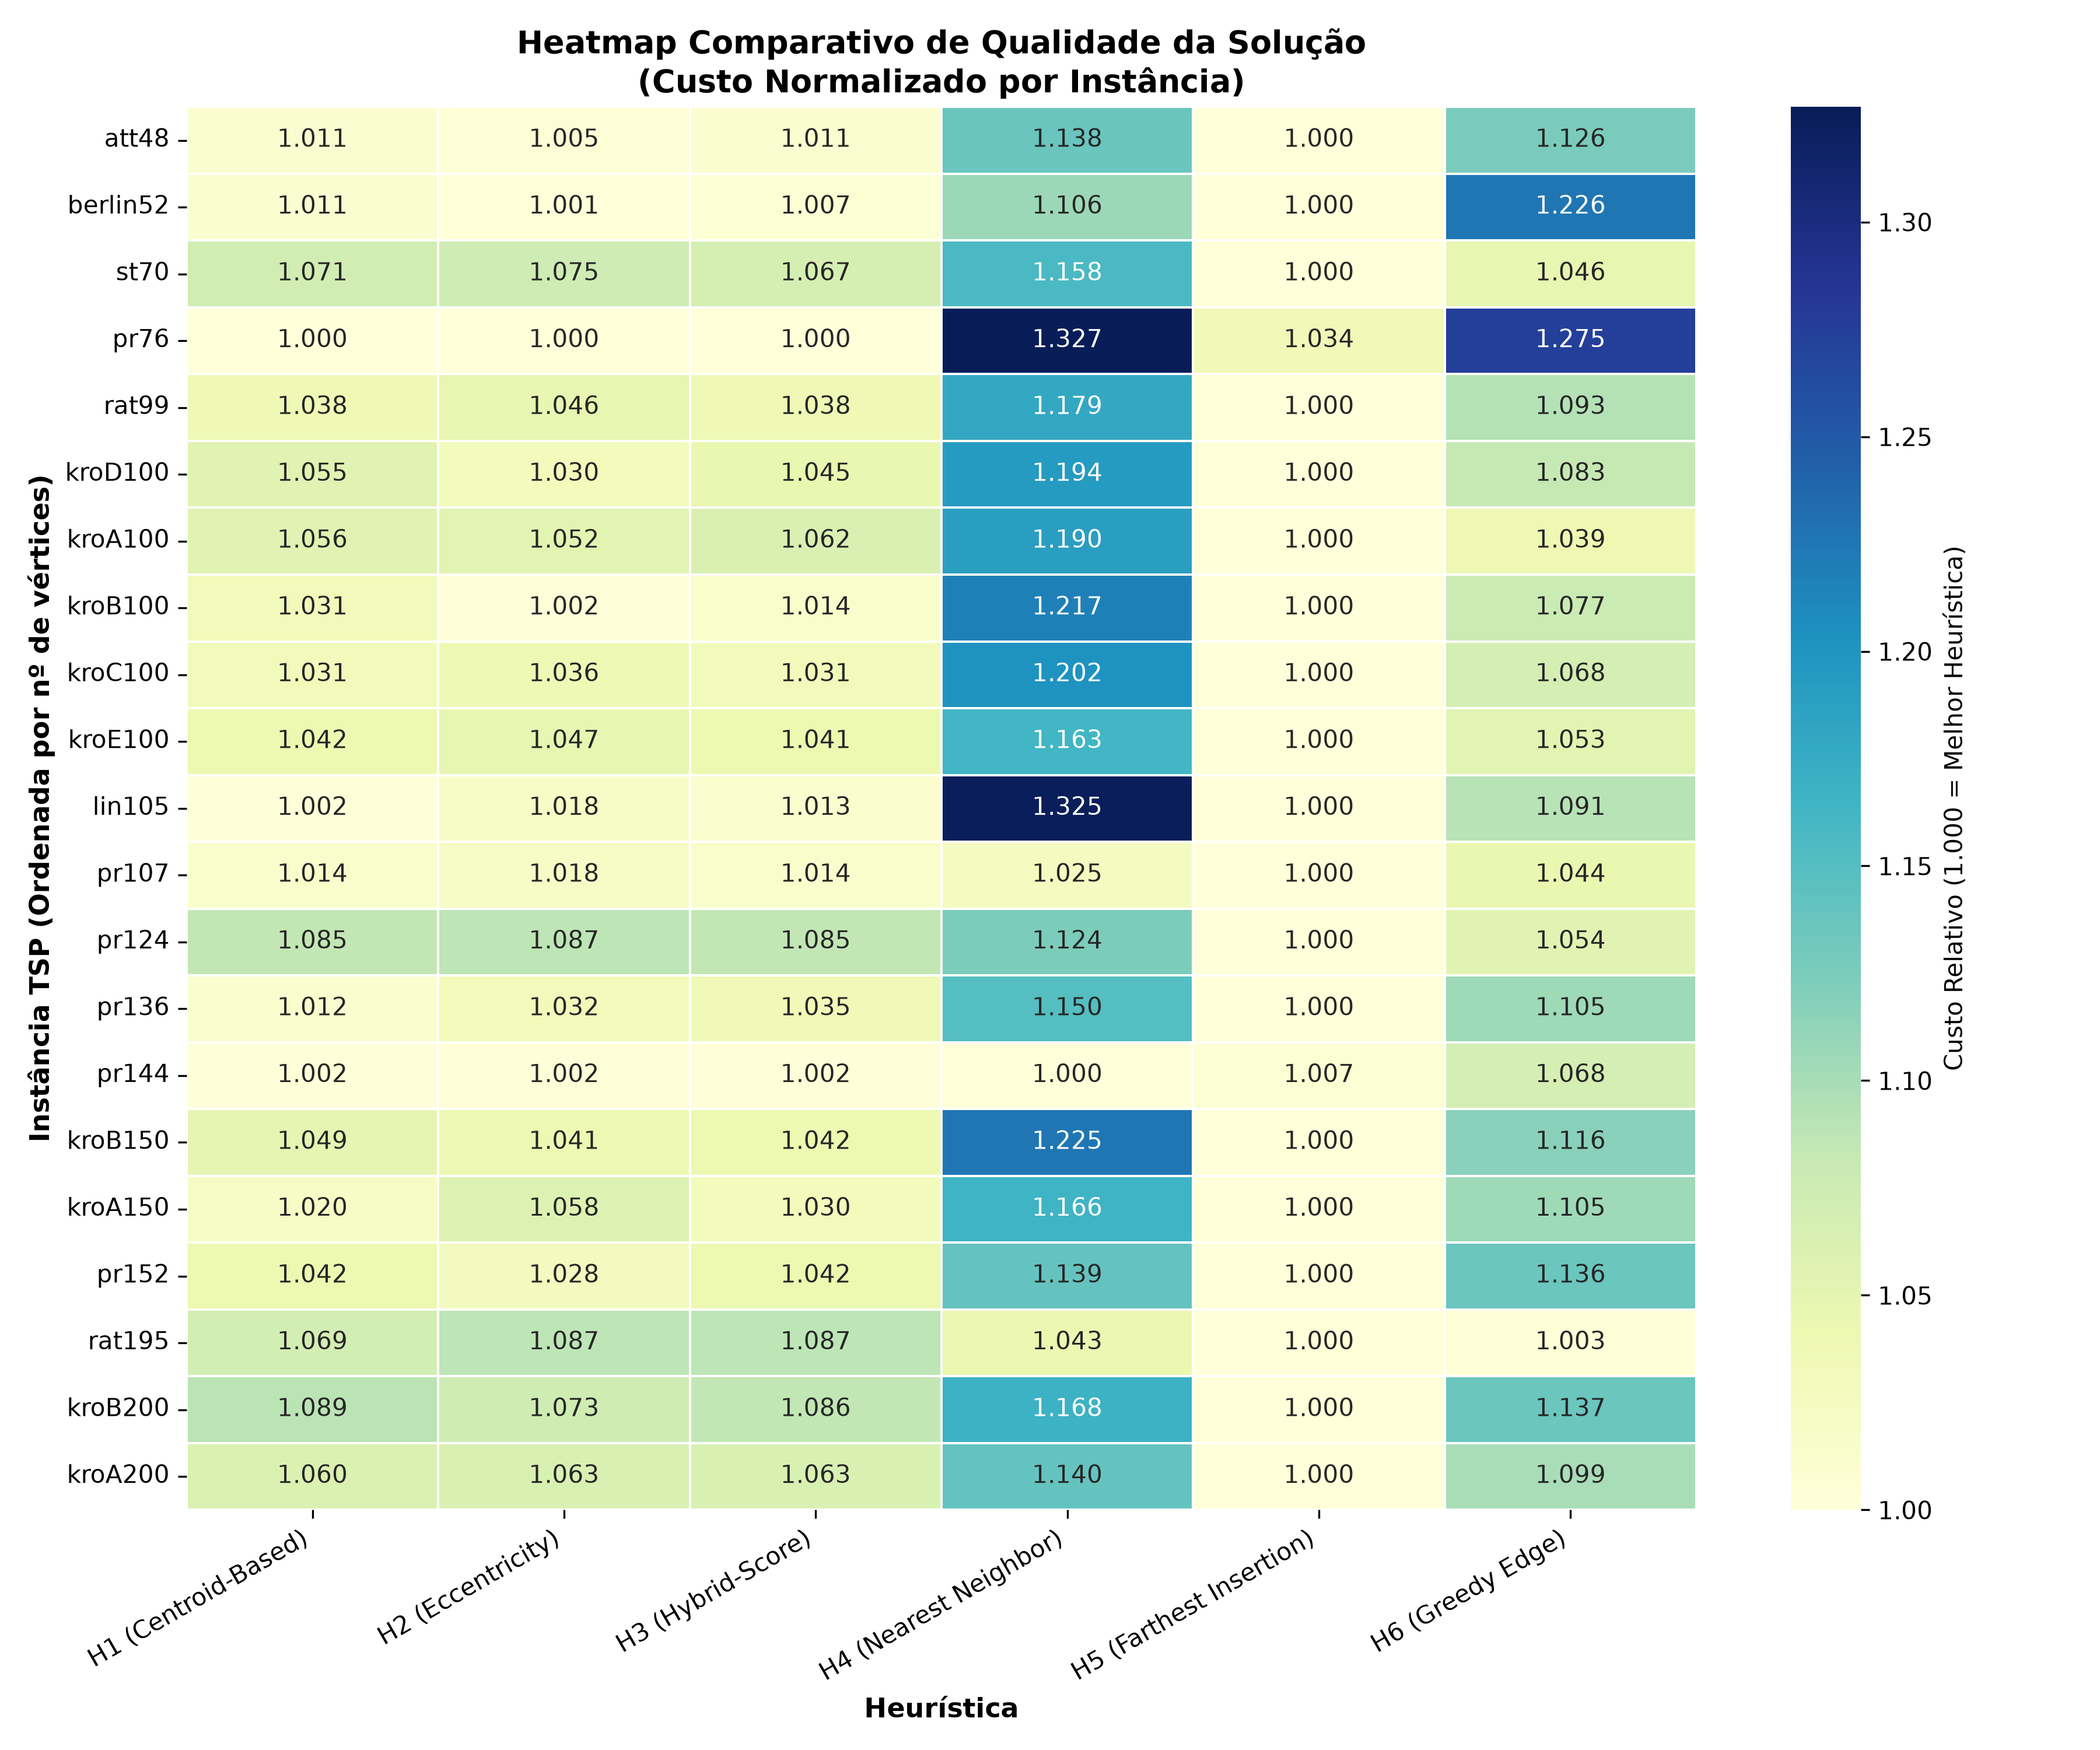
\includegraphics[width=1\textwidth]{heatmap_custo_relativo.png}
    \caption{\textit{Heatmap} do Custo Relativo por instância e heurística. Tons mais
    claros indicam desempenho mais próximo de $1{,}000$ (melhor solução entre as
    heurísticas testadas naquela instância).}
    \label{fig:heatmap_custo}
\end{figure}

O \textit{heatmap} cruza as 21 instâncias (linhas, ordenadas pelo número de vértices)
com as 6 heurísticas (colunas). A célula $(i, h)$ exibe o Custo Relativo
$\mathrm{CR}(h, \mathcal{I}_i)$, definido na Seção~3. H5 obtém valor $1{,}000$ na
grande maioria das instâncias. As heurísticas autorais H1, H2 e H3 operam
consistentemente na faixa entre $1{,}01$ e $1{,}09$, superando com folga H4 e H6.

\subsection{\textit{Heatmap} de Tempo Computacional}

\begin{figure}[H]
    \centering
    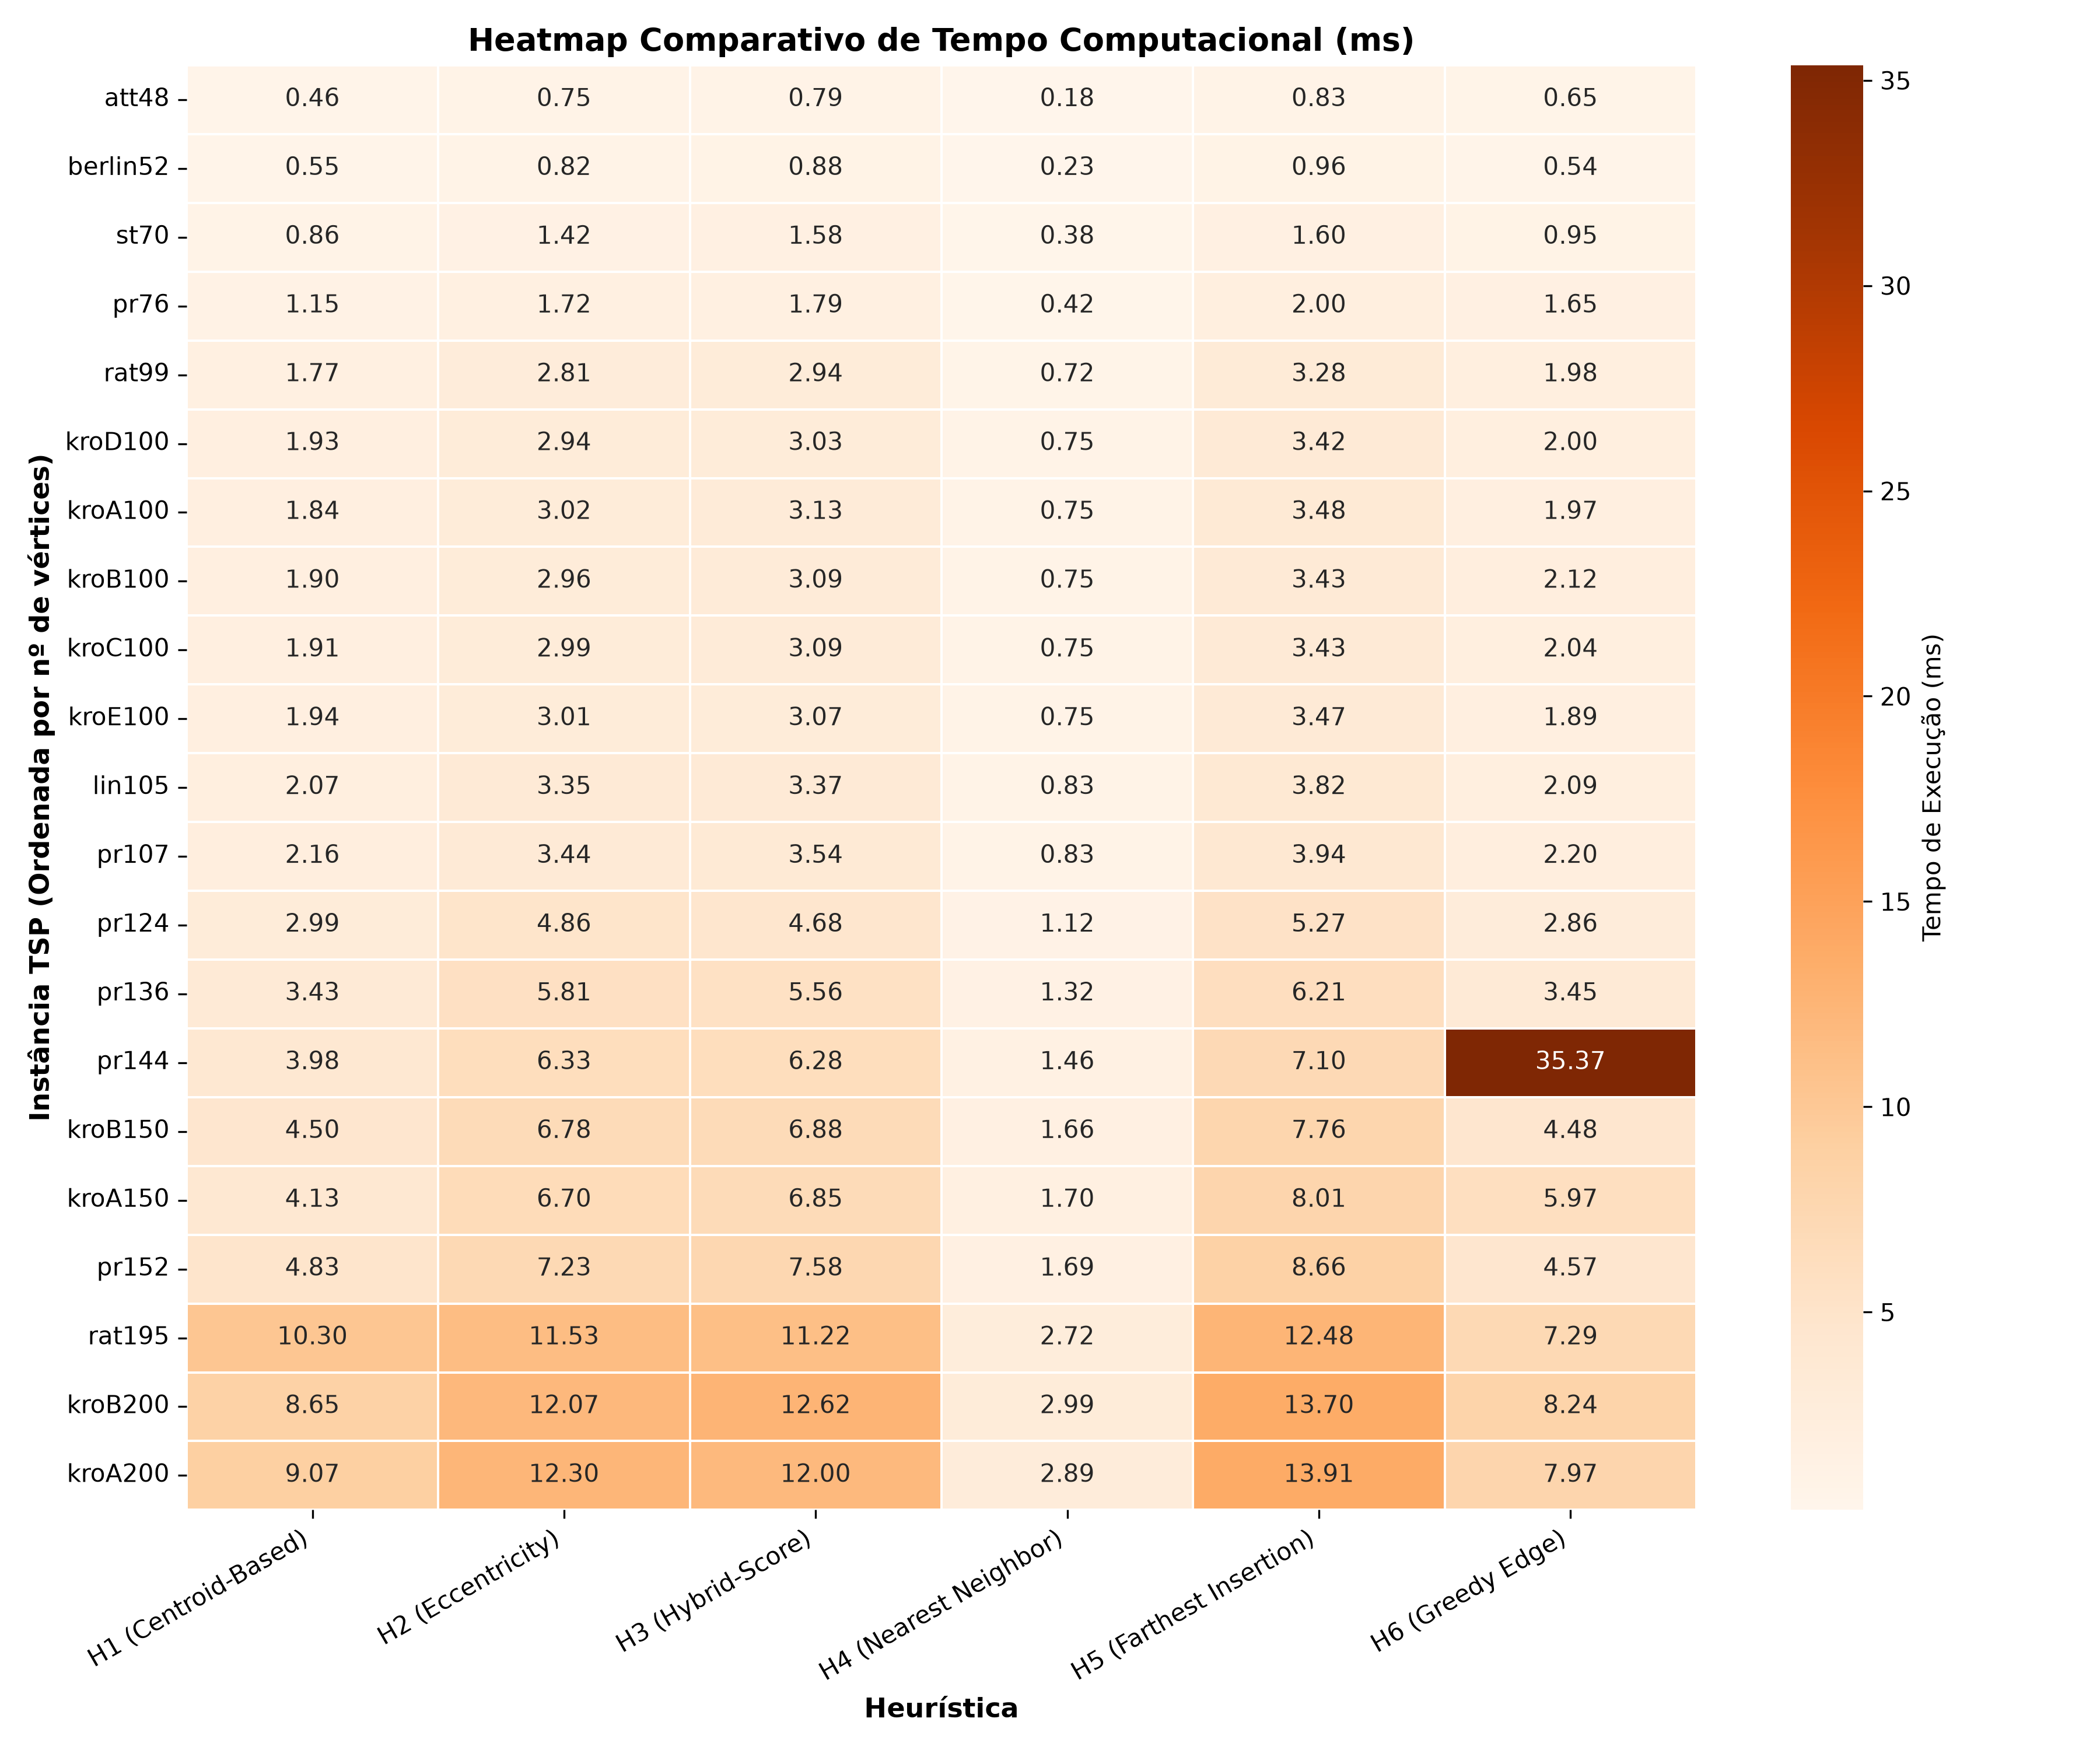
\includegraphics[width=1\textwidth]{heatmap_tempo_execucao.png}
    \caption{\textit{Heatmap} do tempo de execução em milissegundos por instância e
    heurística.}
    \label{fig:heatmap_tempo}
\end{figure}

Permite verificar visualmente como a complexidade de cada heurística escala com o
aumento de $n$. H4 mantém-se abaixo de $3\,ms$ mesmo para $n = 200$. H1 apresenta
clara vantagem de velocidade sobre H2, H3 e H5 nas instâncias maiores: o cálculo do
centróide é $O(n)$, ao passo que o cômputo da excentricidade e o critério de seleção do
\textit{Farthest Insertion} exigem operações quadráticas contínuas.

\subsection{\textit{Boxplot} de Custo Relativo}

\begin{figure}[H]
    \centering
    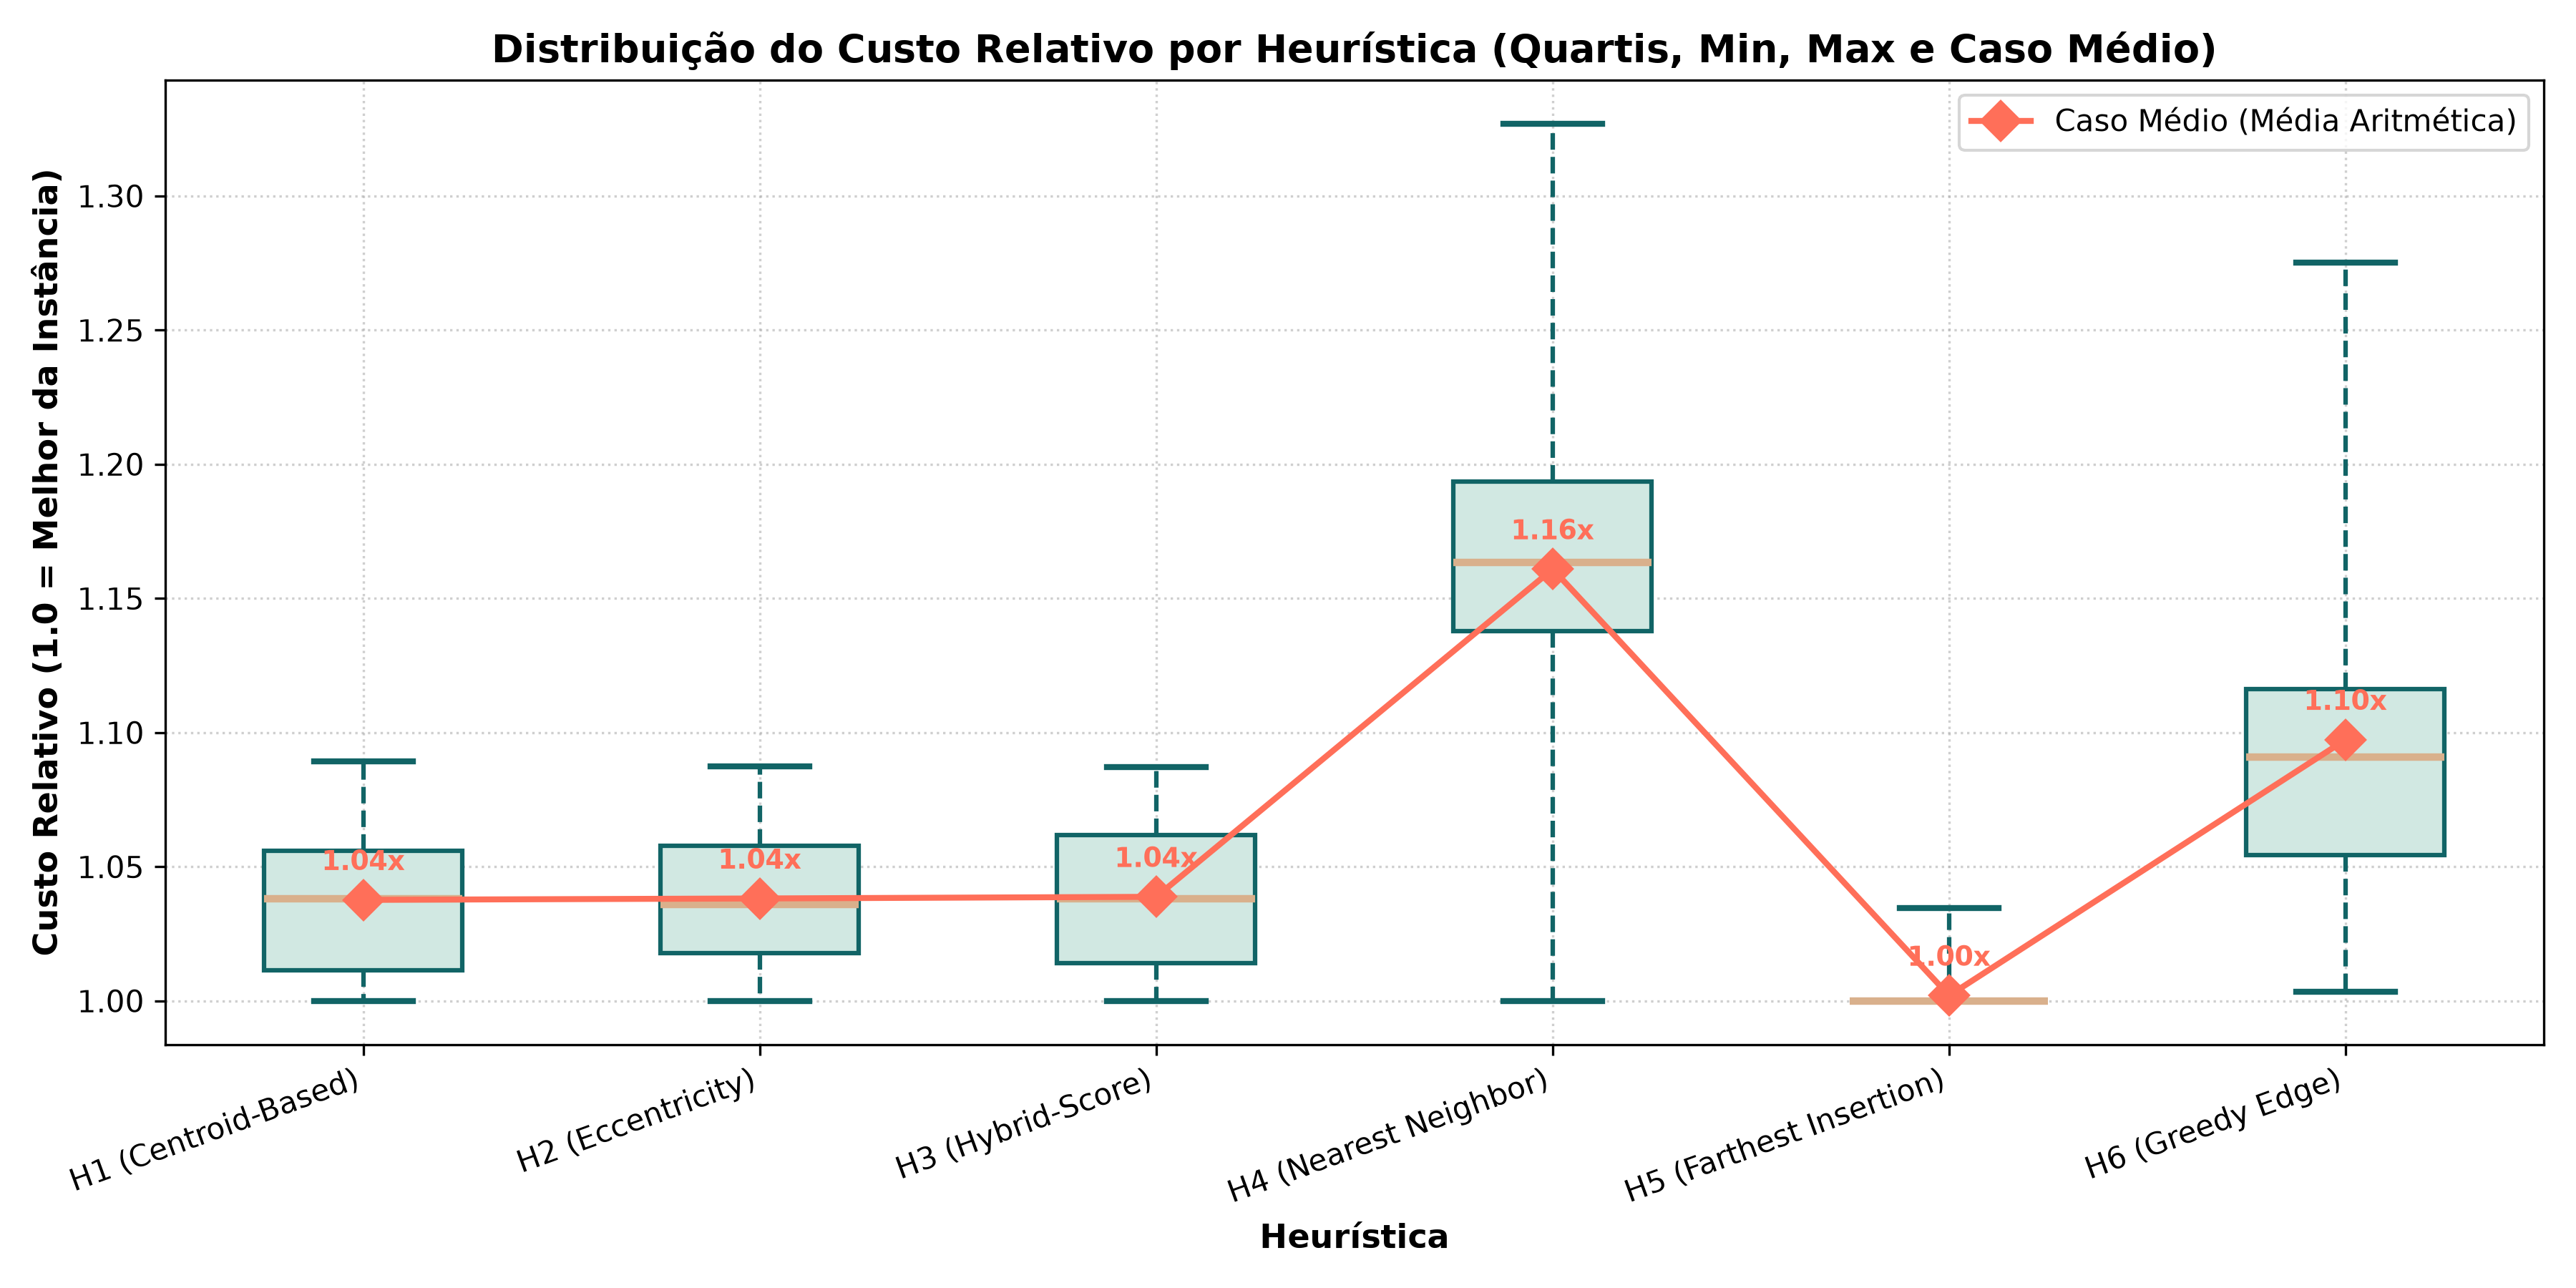
\includegraphics[width=1\textwidth]{boxplot_custo_relativo.png}
    \caption{Distribuição estatística do Custo Relativo por heurística nas 21 instâncias.
    A linha central da caixa indica a mediana; a linha laranja com diamantes indica a
    média aritmética.}
    \label{fig:boxplot_custo}
\end{figure}

O gráfico exibe, para cada heurística, a distribuição do Custo Relativo
$\mathrm{CR}(h, \mathcal{I}_i)$ sobre as 21 instâncias. A caixa é delimitada pelo
primeiro quartil (Q1) e pelo terceiro quartil (Q3); os \textit{whiskers} estendem-se do
mínimo ao máximo observado. A linha laranja com diamantes sobrepõe explicitamente a
média aritmética. H1, H2 e H3 apresentam caixas estreitas, indicando baixa
variabilidade e previsibilidade de qualidade. H4 e H6, por sua vez, exibe dispersão ampla e
cauda longa de soluções piores.

\subsection{\textit{Boxplot} de Tempo de Execução}

\begin{figure}[H]
    \centering
    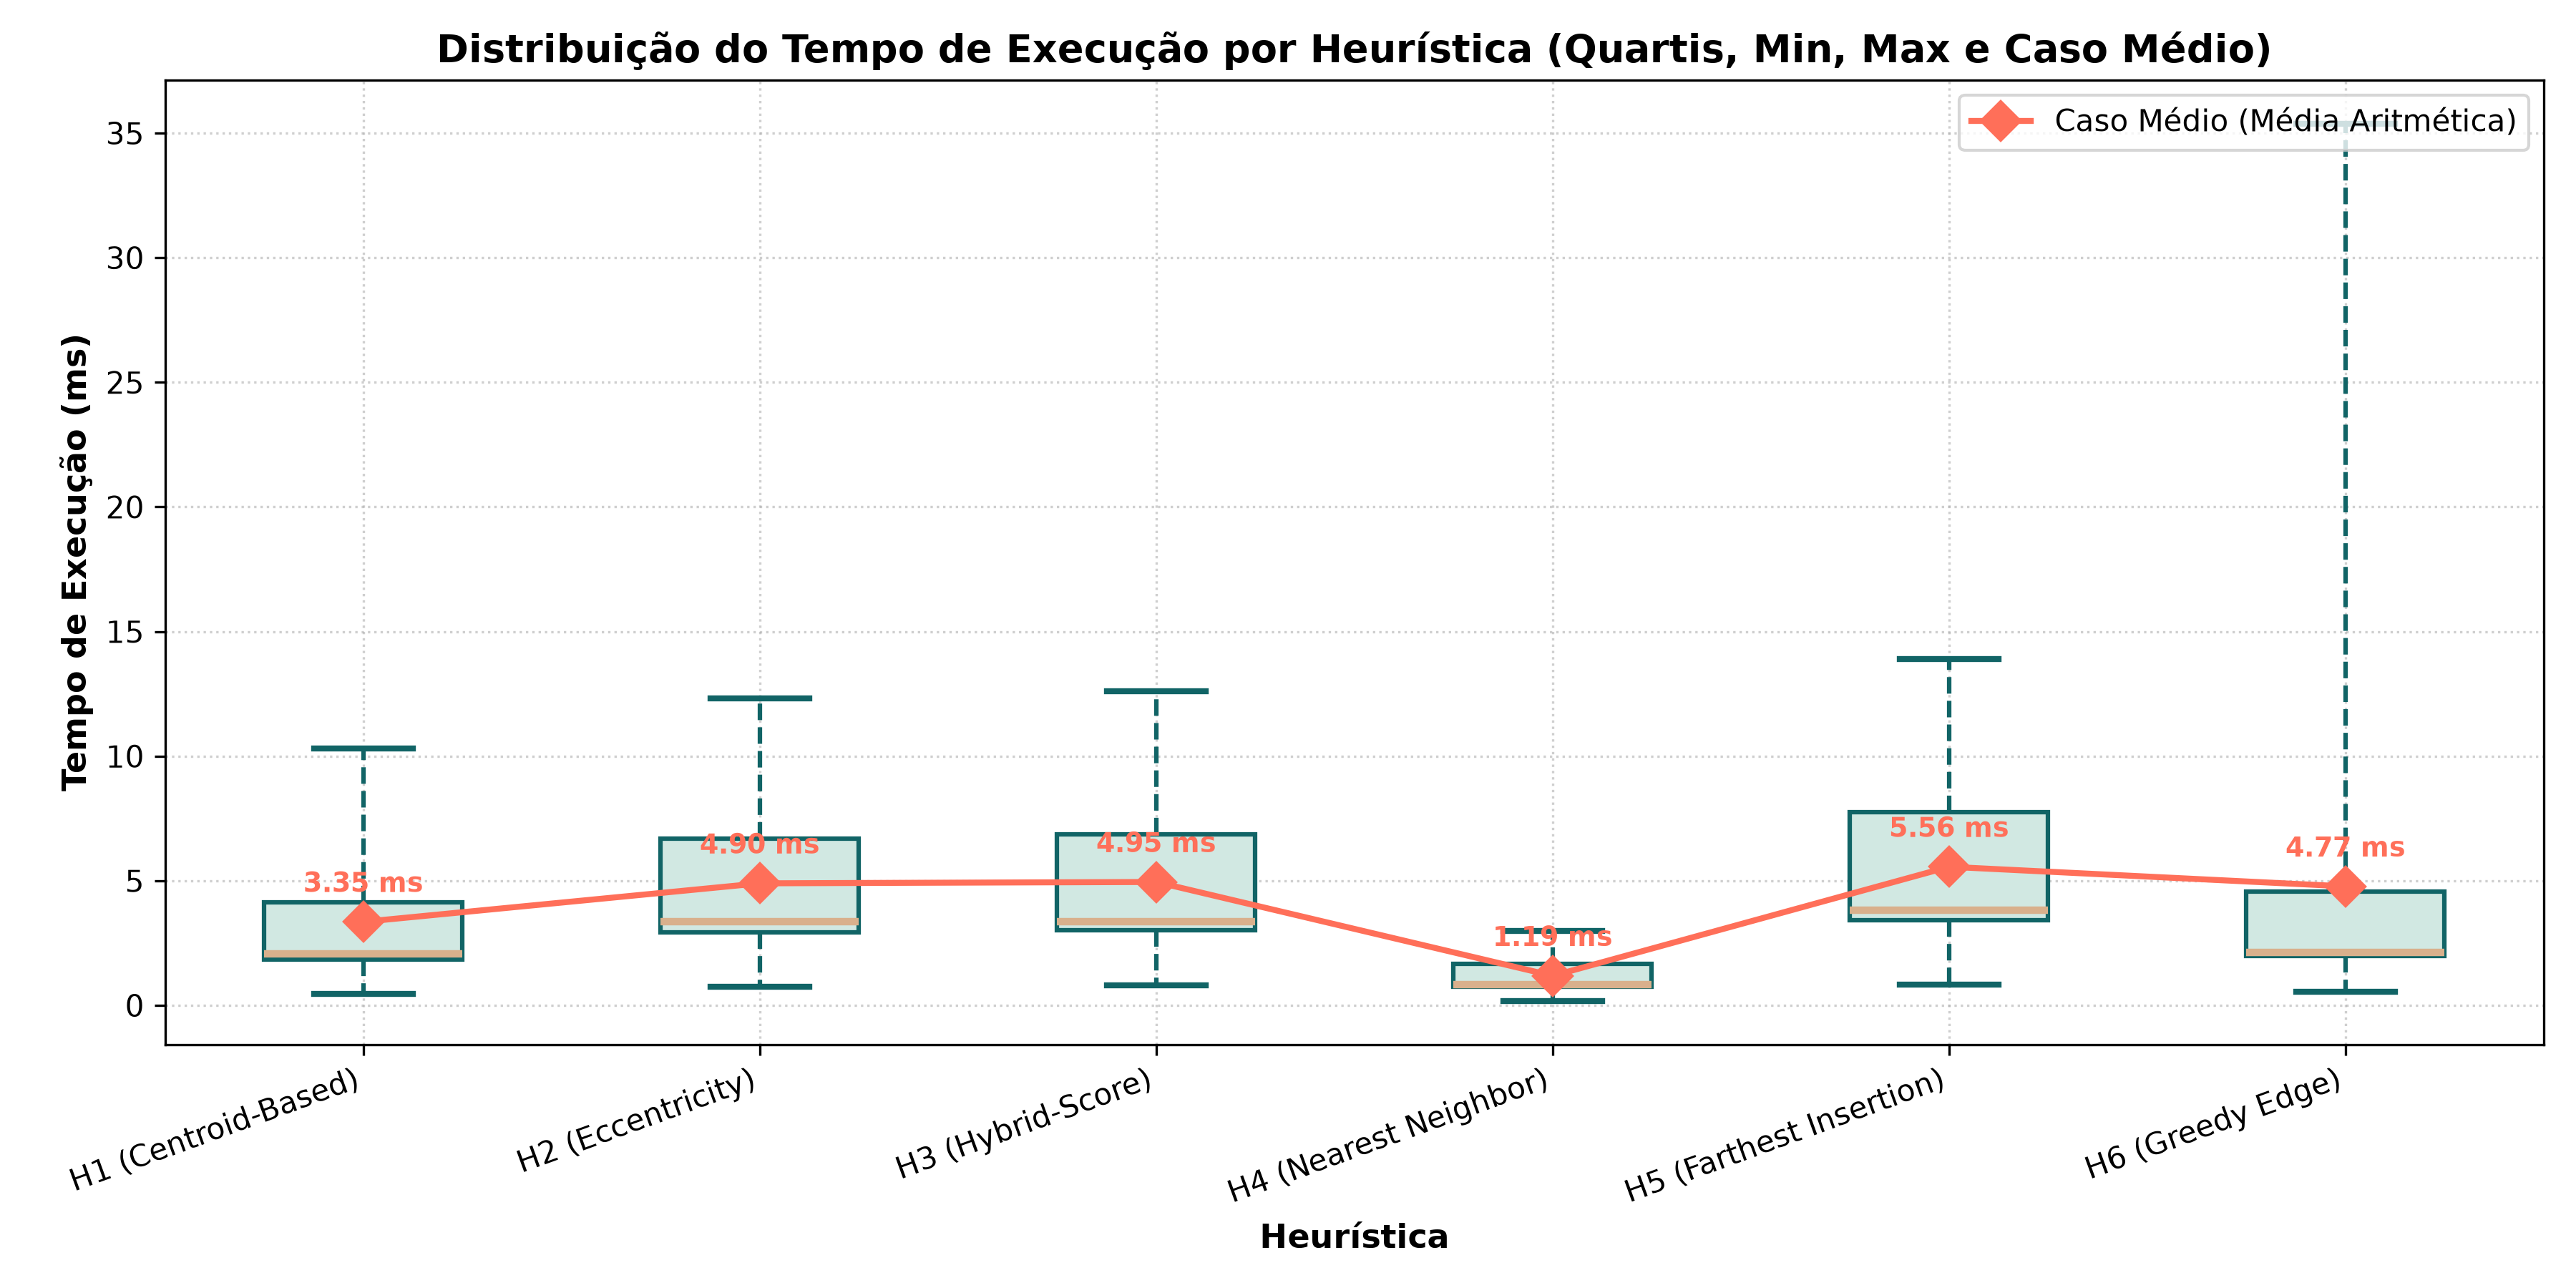
\includegraphics[width=1\textwidth]{boxplot_tempo_execucao.png}
    \caption{Distribuição estatística do tempo de execução (ms) por heurística.}
    \label{fig:boxplot_tempo}
\end{figure}

Ilustra a estabilidade dos tempos de execução entre instâncias e confirma a vantagem
de velocidade de H1 em relação a H5 e H2, sem sacrifício expressivo de qualidade.

\subsection{Fronteira de Pareto Multiobjetivo}

\begin{figure}[H]
    \centering
    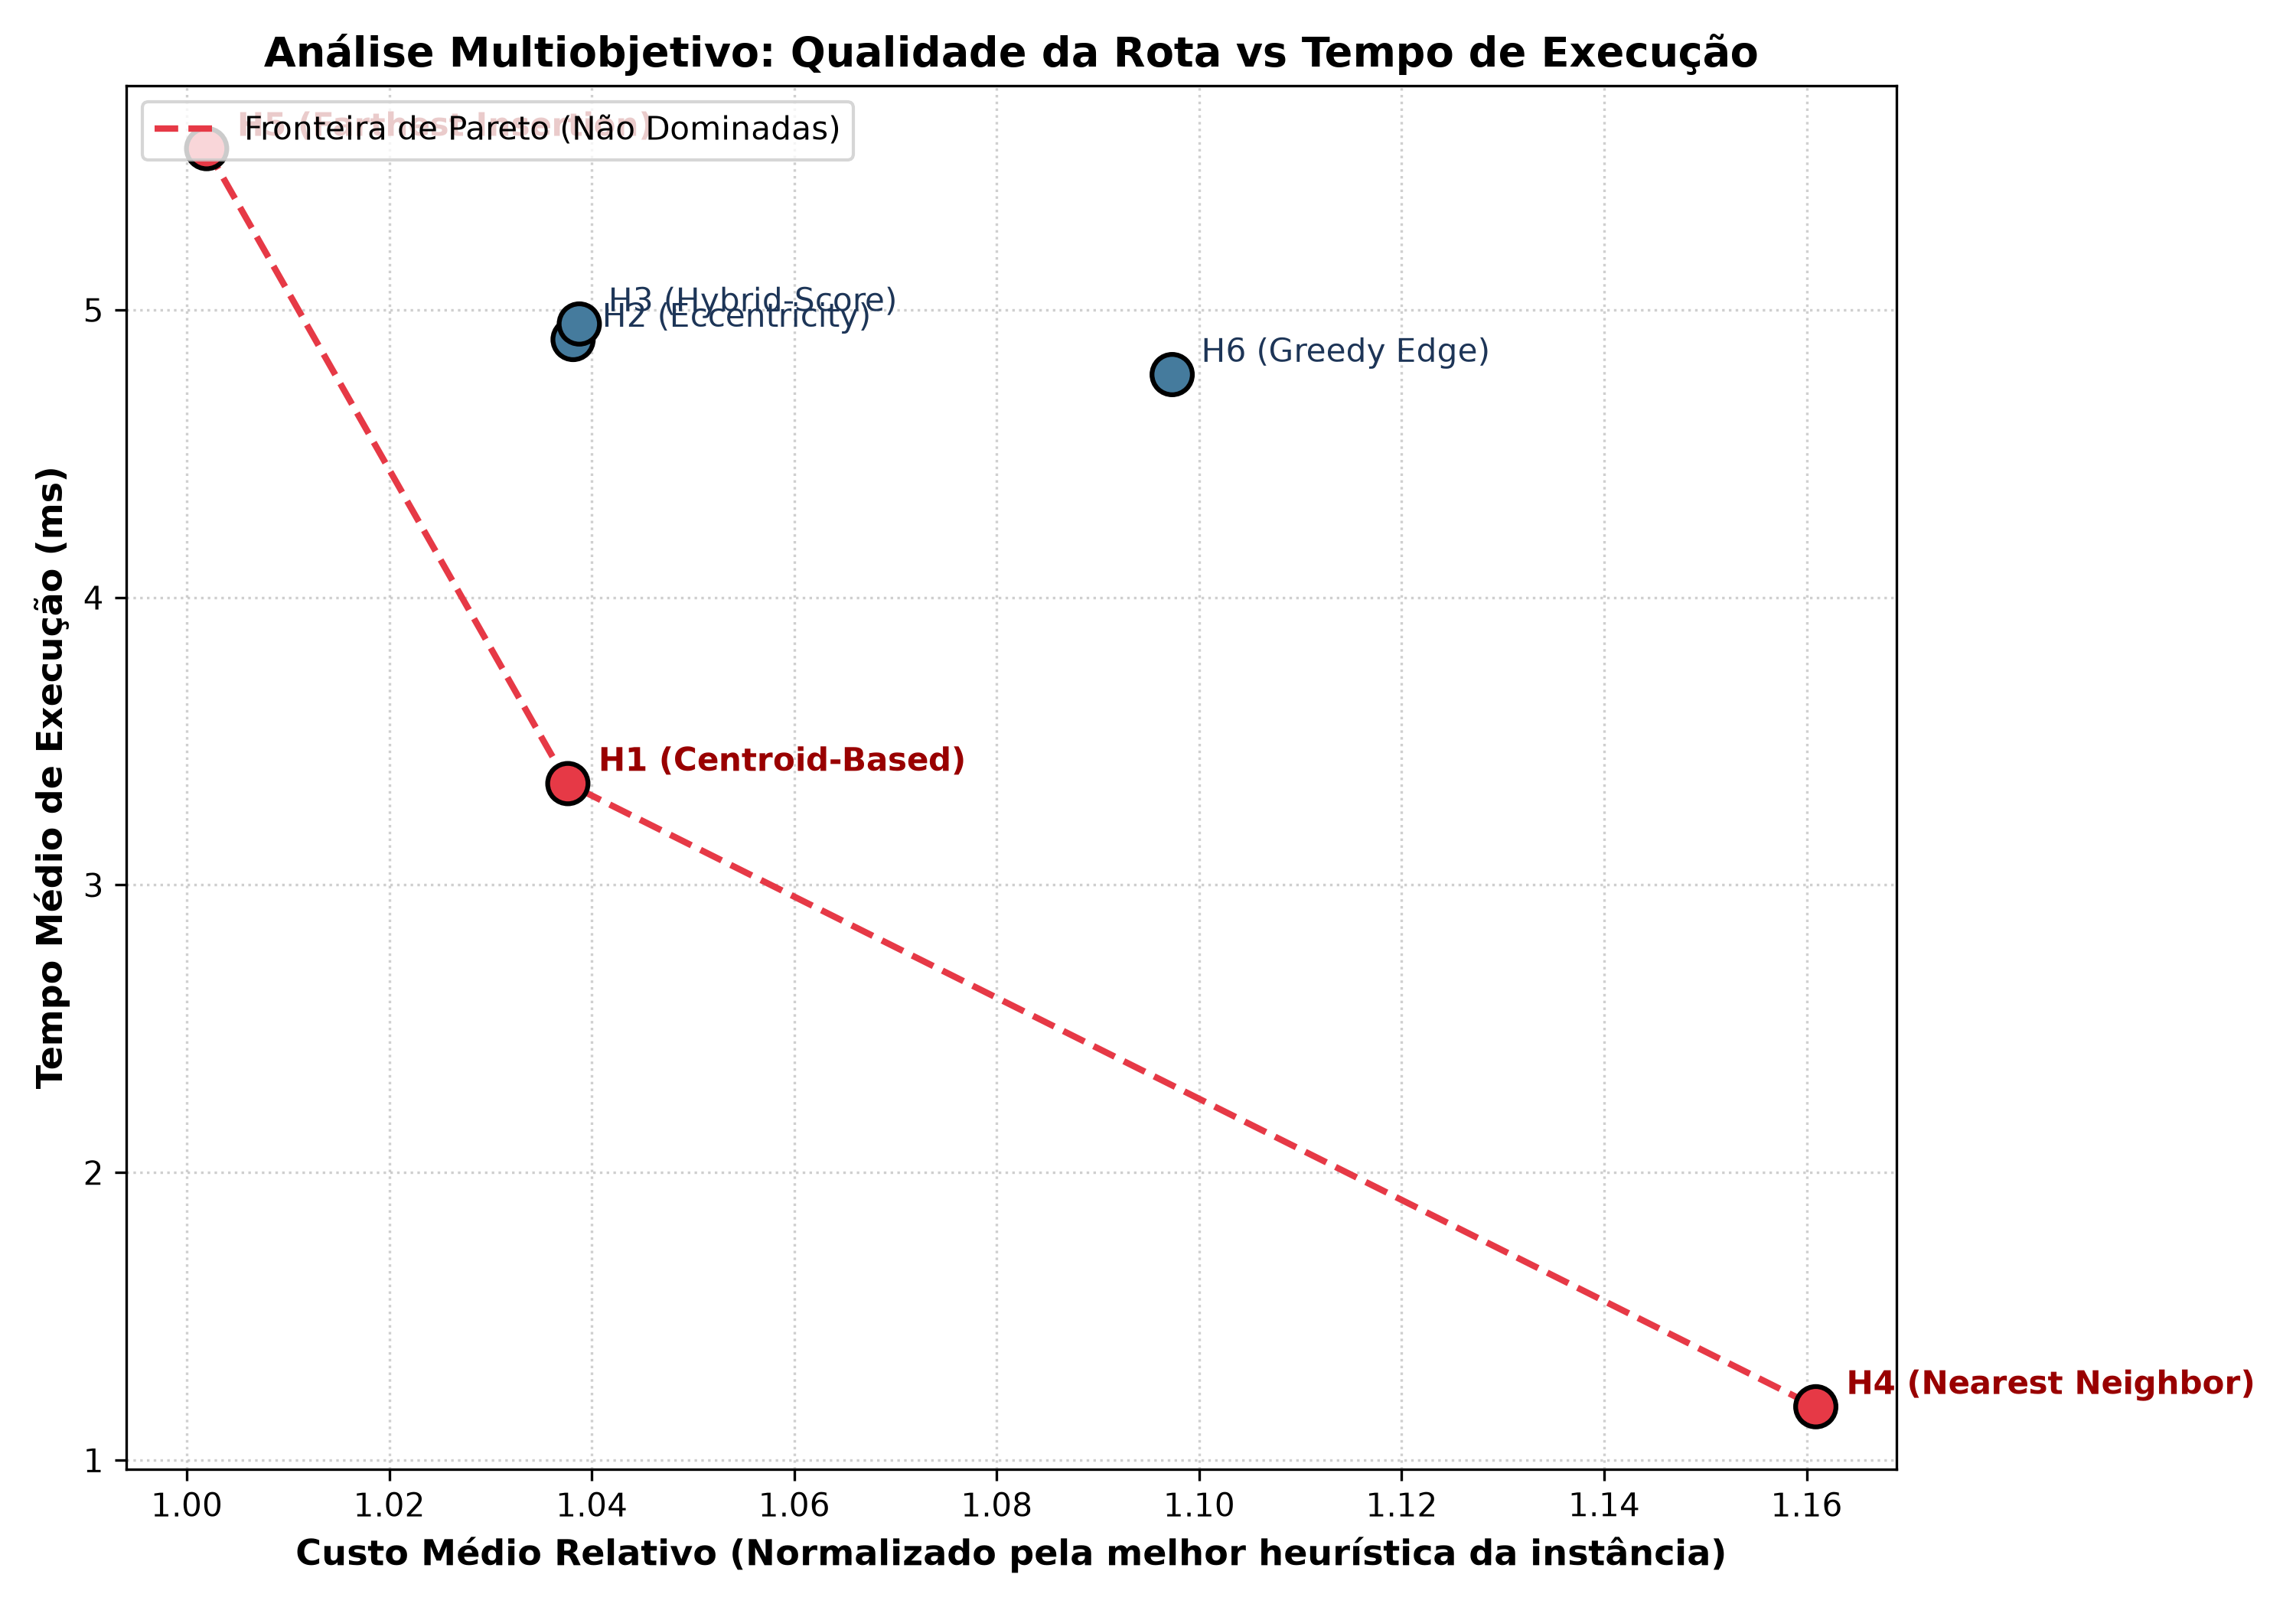
\includegraphics[width=1\textwidth]{fronteira_pareto.png}
    \caption{Diagrama de dispersão Custo Médio Absoluto $\times$ Tempo Médio de Execução.
    Pontos vermelhos conectados pela linha tracejada compõem a Fronteira de Pareto
    (soluções não dominadas).}
    \label{fig:pareto}
\end{figure}

O diagrama relaciona os dois objetivos conflitantes: minimizar o custo do circuito e
minimizar o tempo de execução. As soluções não dominadas formam a Fronteira de Pareto,
destacadas em vermelho:

\begin{itemize}
    \item \textbf{H4 (\textit{Nearest Neighbor})}: escolha ótima quando a prioridade
          absoluta é latência mínima.
    \item \textbf{H1 (\textit{Centroid-Based})}: ponto de inflexão da curva ---
          entrega qualidade próxima à de H5 com aproximadamente metade do tempo
          computacional, configurando o melhor \textit{trade-off} geral.
    \item \textbf{H5 (\textit{Farthest Insertion})}: escolha ótima quando a prioridade
          absoluta é a qualidade da rota, aceitando maior custo computacional.
\end{itemize}

As heurísticas H2, H3 e H6 ficam no interior dominado da fronteira, ou seja, para cada
uma delas existe ao menos uma heurística na fronteira que as supera simultaneamente em
custo e em tempo.

% -------------------------------------------------------
% Referências
% -------------------------------------------------------
\bibliographystyle{plain}
\bibliography{referencias}

\end{document}